\chapter{Requirement specification}
\section{Purpose and scope}
Formål og omfang samt anvendelse.
\section{References}
Referencer
\section{Glossary}
Ordforklaringer
\section{General description}
\subsection{General System}
\begin{figure}[H]
	\centering
	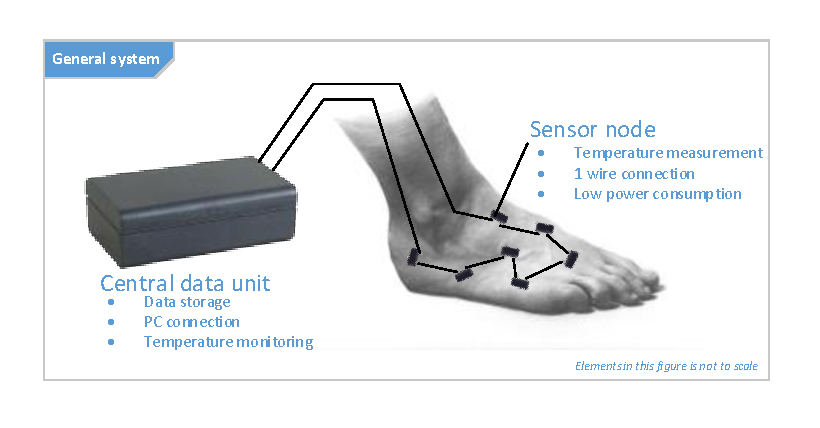
\includegraphics[width=0.8\textwidth]{billeder/GeneralSystem}
	\caption{General System}
\end{figure}

\subsection{System description}
Et device der skal påmonteres foden på en person der er disponeret til at udvikle Charcotfod. Devicet skal ud fra temperatur og aktivitetsniveau finde ud af om der er en fare for overbelastning. Hvis dette er tilfældet skal brugeren advares.

%\subsection{Prototype af UI eller GUI}

%\subsection{Beskrivelse af UI eller GUI}

\section{Functional requirements}

\subsection{System Features}

\subsubsection{Feature 1}

\subsubsection{Feature 2}

\subsection{Additional Features}

\subsubsection{Feature 1}

\subsubsection{Feature 2}

\section{Non functional requirements}

\subsection{General requrements}

\subsection{Temperature sensor requirements}

\subsubsection{Functionality Requirements}

\subsubsection{Hardware Requirements}
Krav til hardware (if any)\\
*Power consumption\\
*Performance\\
*Maintainability\\
*Interfaces\\
*Accuracy\\
\subsubsection{Software Requirements}
Krav til software (if any)\\
*Performance\\
*Maintainability\\
*Interfaces\\
*Language??\\

\subsubsection{External interfaces}
N/A
\subsection{Main data collection unit requirements}

\subsubsection{Functionality Requirements}

\subsubsection{Hardware Requirements}
Krav til hardware (if any)\\
*Power consumption\\
*Performance\\
*Maintainability\\
*Interfaces\\
*Accuracy\\

\subsubsection{Software Requirements}
Krav til software (if any)\\
*Performance\\
*Maintainability\\
*Interfaces\\
*Language??\\

\subsubsection{External interfaces}
*USB?\\
*UART?\\
*EEPROM?\\
*Flash?\\

\subsection{Project requirements}

\subsubsection{Documentation}
\begin{itemize}
\item Engelsk
\item SysML
\end{itemize}

\subsubsection{Technologies and tools}
\begin{itemize}
\item Matlab
\item Maple/Mathcad
\item Microsoft Visio 2010/2013
\item TortoiseSVN
\item TeXmaker
\end{itemize}

\subsubsection{Misc}
\begin{itemize}
\item Report is written in LaTeX.
\end{itemize}

\section{Non functional requirements}
(?) betyder at jeg ikke lige ved hvordan det skal specificeres eller om det overhovedet er et reelt krav.\\
\subsection{system requirements }
%%%%%%%%%%%%%%%%%%%%
% Generelle krav %
%%%%%%%%%%%%%%%%%%%%
General Requirements:\\
\begin{itemize}
\item Systemet skal have en levetid på 1-3 år(specificitet)
\item Der skal tænkes på fremstillingspris(?)
\end{itemize}
%%%%%%%%%%%%%%%%%%%%
% Sensor krav %
%%%%%%%%%%%%%%%%%%%%
Sensor requirements:\\
\begin{itemize}
\item Målesensoren skal have en nøjagtighed på $\pm0.5 ^{\circ}C$
\item Accelerometer
\item Kalibrering(?)
\end{itemize}
%%%%%%%%%%%%%%%%%%%%
% Central dataopsamling%
%%%%%%%%%%%%%%%%%%%%
Central data collection unit:\\
\begin{itemize}
\item Clock speed
\item GPIO amount
\end{itemize}

%Teksturdesign:\\
%\begin{itemize}
%\item Sokken skal være meget elastisk(?)
%\item Sokken skal kunne anvendes hele dagen(?)
%\item Sokken skal kunne avnendes med fodtøj(?)
%\item Sokken skal kunne rengøres (?)
%\end{itemize}

\subsection{Communication requirements}
\begin{itemize}
\item 0 - 12 VDC $\pm$0.5VDC
\item 500 mA $\pm$25mA
\end{itemize}

\subsection{Interfaces Requirements}
prototyper af PC og/eller smartphone\\
Datastik så data kan tages ud af enheden for debugging purpose.\\

\subsection{Development and technology requirements }
V-model:\\
\begin{itemize}
\item Modificeret Scrum til styringsprocessen for sprint mellem hver projektmilestone
\item Henvisning til tidsplan og milestones
\end{itemize}

Documentation:\\
\begin{itemize}
\item Engelsk
\item SysML
\end{itemize}

Technologies and tools:\\
\begin{itemize}
\item Matlab
\item Maple/Mathcad
\item Microsoft Visio 2010/2013
\item TortoiseSVN
\item TeXmaker
\end{itemize}

Misc:\\
\begin{itemize}
\item Report is written in LaTeX.
\end{itemize}
\section{List of figures}